\subsection{Management and organization}
As a start up company progresses, resources and workforce increase. To ensure responsibilities and daily tasks a hierarchy can be structured within the company. Ground rules has to be set in the start of such process because later discussions and arguments can happen between the owners. Below is a description of the organisational structure, ownership and key activities- and resources.

\subsubsection{Legal structure and ownership}
The concept is an equally owned idea between the group members. It has been declared since the beginning of the project in the group contract.
Since the group consist of students, the project will require funding to become a reality. No one is interested in being personally liable for the debt if the company should go bankrupt. That is why creating an ApS would be a good option. This requires at least 50.000 kr. of value (can be values of objects too) to settle. The risk of doing it this way is that the investors will probably force the group members to sign for a personal liable agreement. 
When investors act, the ownership will probably change also as they will be a part of it.
\todo[inline, color=red!50]{Going once, Going twice...}
\thomas{Going third...? What does this mean?}
\subsubsection{Management}
A conclusion has been drawn from the Belbin group result. It is based on the requirements of the different titles within the company.  For instance, we felt that the CEO would require a strong represent who has a great overview (Acts as a coordinator), a talent for communication (Resource Investigator) and the drive of a shaper. Within these three fields, a score was created based on the individual Belbin results, which lead to choosing David as the CEO. 
The same procedure was followed when assigning candidates for the other posts. 
% \begin{itemize}
% \item CEO, David
% \item CTO, Xabier
% \item CFO, Casper
% \end{itemize}

Nikolaj, Thomas, David and Kirstine is chosen as the implementers as they are best suited for programming and making the sensor.
It is obvious from figure \ref{management_structure} that our management structure is heavily based on development and thus the chief technical officer is a very key role in this type of company.

\begin{figure}[ht]
\centering
    \tikzstyle{mp} = [font=\footnotesize, draw, rectangle, fill=blue!10, text=black, text width = 3.7em, minimum height =4.1em, text centered]
  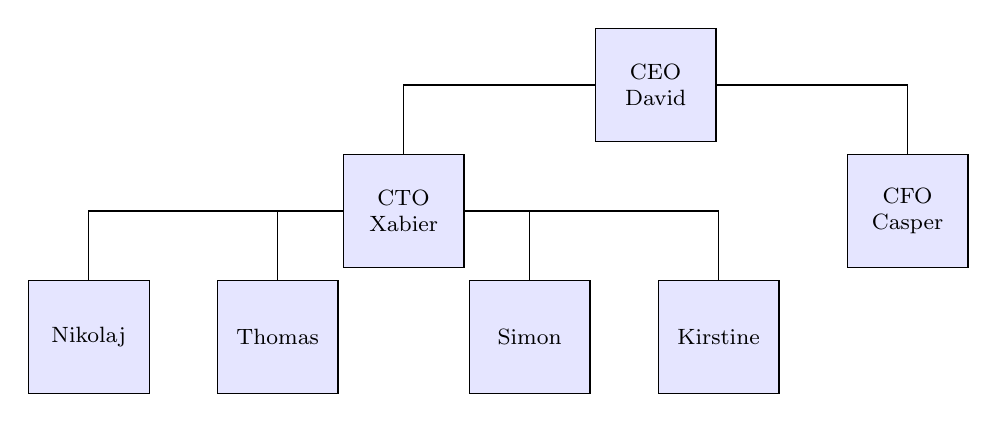
\begin{tikzpicture}[scale=0.8]
  \draw (0,0)
  node[mp] (ceo)                     {CEO\\David} 
  (ceo) -| ++(-4,-2) node[mp] (cto)  {CTO\\Xabier} 
  (ceo) -| ++( 4,-2) node[mp] (cfo)  {CFO\\Casper}
  
  (cto) -| ++(-5,-2) node[mp] (impA) {Nikolaj}
  (cto) -| ++(-2,-2) node[mp] (impb) {Thomas}
  (cto) -| ++( 2,-2) node[mp] (impc) {Simon}
  (cto) -| ++( 5,-2) node[mp] (impd) {Kirstine}
  ;  
  \end{tikzpicture}
  \caption{Management structure of Interflex}
  \label{management_structure}
\end{figure}


\subsubsection{Board and advisors}
As usual, the leaders of a company will be sitting within the board, but different partners would also play a big role within. If a company decides to buy our product, for using it in their own solutions, they could have an interest of being a board member. Because they can try to make the development of the product go a direction of their choice. In the end they are the ones who sell to the end customers and if they don't have any sales, our company makes no profit either. So having them influence the product and development could benefit both of us. 
It could be interesting to have other partners within the board, especially some within the technological field, robot- and software wise.
One of the most valuable advisors to have would be a person with experience within innovation and technology, who also has experience with a start up company. 

\subsubsection{Partnerships}
The strategy of the company relies on having different distributors within Europe, therefore it is essential to have partnerships with these companies. They are not the final customer of our company, but a link to them. This is where the main revenue streams are going to be created.
For instance, Valk Welding would be an optimal partner within the Danish market, since they are able to reach the final customers within Denmark. It is our goal to reach distributors like Valk Welding within the european market.
Another sort of interesting partners is one of the majors of the market. This could be Migatronic, Valk Welding, Universal Robots or any other sort of major company within the field of welding technology, who already exist on the market. The reason for this is that they could be interested in the technology our product offers and that they would like to integrate it within their range of products. This situation would usually lead to them investing in our company and putting a limit to which companies we are allowed to collaborate with.

\subsubsection{Key activities}
For the project to become a reality it would require financing, unless the group members settles for working on the project through a period of their masters. This would result in a different direction of development, than with a basis capital. Because software is doable without the need of an investment, but when it comes to combining the hardware and software for testing purposes, it is going to require an injection of funds. In this case, the obvious choice would be the group trying to find investors.

Therefore the development of concept is crucial for the company while pitching the idea for potential investors. Other key activities will include the process of combining software and hardware and further testing to improve the product. 

The production phase can begin when a design is done and a stable software release is ready. 

\subsubsection{Key resources}
The key resources are the assets to the company that are necessary to create value for the customer. These shall support the company and make it sustainable.
To summarize the primary key resources to the company:
\begin{itemize}
\item Injection of funds
\item Accommodations for office and development usage
\item Getting the product patented
\end{itemize}
